\documentclass[10pt,journal]{IEEEtran}

\usepackage{amsmath}
\usepackage{booktabs}
\usepackage{graphicx}
\usepackage{microtype}
\usepackage[hidelinks]{hyperref}
\usepackage[capitalise,noabbrev]{cleveref}
\usepackage{balance}

\newcommand{\AFLFPSamples}{1,136}
\newcommand{\AFLFPDetection}{100.0\%}
\newcommand{\AFLFPNMEMean}{6.368\%}
\newcommand{\AFLFPNMEStd}{0.399\%}
\newcommand{\AFLFPNMEMedian}{6.361\%}
\newcommand{\AFLFPNMEP}{6.909\%}
\newcommand{\AFLFPFPS}{24.96}
\newcommand{\AFLFPHardest}{tight eyes closure}
\newcommand{\AFLFPEasiest}{right wink}
\newcommand{\DISFASamples}{5,400}
\newcommand{\DISFADetection}{100.0\%}
\newcommand{\DISFAFOne}{0.714}
\newcommand{\DISFAICC}{0.467}
\newcommand{\DISFAFPS}{26.14}
\newcommand{\DISFABestAU}{AU25}
\newcommand{\DISFAWorstAU}{AU20}
\newcommand{\DISFAPrevalenceCorrelation}{0.708}
\newcommand{\PyFeatVersion}{2.0.3}


\hypersetup{
  pdftitle={Test-Only Evaluation of Py-Feat Detectorv2 on AFLFP and DISFA},
  pdfauthor={Anonymous Author(s)},
  pdfsubject={Reproducible test-only facial behavior benchmark}
}

\newcommand{\code}[1]{\texttt{#1}}
\newcommand{\nme}{\operatorname{NME}}

\title{Test-Only Evaluation of Py-Feat Detectorv2 on AFLFP Landmark
Localization and DISFA Action Units}

\author{Anonymous Author(s)}

\markboth{Independent Py-Feat Benchmark Report, July 2026}%
{Anonymous Author(s): Test-Only Evaluation of Py-Feat Detectorv2}

\begin{document}

\maketitle

\begin{abstract}
Pretrained facial behavior toolkits are frequently used outside the datasets
on which their components were developed, yet deployment-oriented,
test-only measurements are often unavailable for specialized populations.
We evaluate the Py-Feat \code{Detectorv2} pipeline without fitting,
fine-tuning, calibration, or threshold selection on two complementary
benchmarks. The AFLFP cohort contains \AFLFPSamples{} facial-landmark images,
balanced across 88 subjects and 16 movements; landmark localization reaches a
\AFLFPDetection{} detection rate and \AFLFPNMEMean{} mean normalized mean
error (NME). The DISFA cohort contains \DISFASamples{} spontaneous
left-camera frames, uniformly balanced at 200 frames for each of 27 subjects;
action-unit detection reaches \DISFADetection{} detection, macro F1
\DISFAFOne{}, and macro ICC(3,1) \DISFAICC{}. Inference throughput is
\AFLFPFPS{} frames/s on AFLFP and \DISFAFPS{} frames/s on DISFA on an Apple
M1 Pro using Metal Performance Shaders. AFLFP error is stable across
movements, whereas DISFA performance is heterogeneous: AU25 achieves F1
0.959 and AU20 achieves 0.479. The results establish a reproducible external
baseline for Py-Feat, while exposing class imbalance, intensity-scale
mismatch, and sampling limits that preclude claims of state-of-the-art
superiority.
\end{abstract}

\begin{IEEEkeywords}
action units, AFLFP, DISFA, facial landmarks, facial palsy, Py-Feat,
test-only evaluation
\end{IEEEkeywords}

\section{Introduction}

Facial behavior pipelines combine face detection, geometric localization, and
expression inference behind a convenient interface. Py-Feat is an open-source
toolbox designed to make these components accessible and benchmarkable
\cite{cheong2023pyfeat}. A package-level benchmark, however, does not directly
answer a deployment question: how does the installed pretrained pipeline
behave on a specialized dataset when no task-specific fitting is permitted?

We study that question in two different regimes. AFLFP was designed around
facial palsy and contains asymmetric expressions with 68-point manual
landmarks \cite{xia2023aflfp}. DISFA contains spontaneous video with
frame-level intensities for 12 Facial Action Coding System action units (AUs)
\cite{mavadati2013disfa}. The former evaluates geometry under atypical facial
motion; the latter evaluates expression scores under natural temporal and
class imbalance.

This report makes three contributions. First, it gives an explicitly
\emph{test-only} measurement of Py-Feat \code{Detectorv2}: pretrained weights
are frozen and no parameter, threshold, or sample is selected using benchmark
performance. Second, deterministic cohorts cover every subject and target
class while limiting the computation required by the full video corpus.
Third, aggregate JSON, sample-level CSV, tables, and vector figures form one
auditable chain. Every number in the manuscript is regenerated from the saved
predictions.

The study is an external evaluation, not a new model and not a controlled
leaderboard entry. In particular, ``test-only'' describes the actions
performed in this study; it does not certify that every upstream pretraining
source is disjoint from AFLFP or DISFA.

\section{Benchmarks and Prior Evidence}

\subsection{Py-Feat}

Py-Feat provides a common interface for facial feature detection,
preprocessing, analysis, and visualization \cite{cheong2023pyfeat}. The
evaluated installation is version \PyFeatVersion{}, using the packaged
\code{Detectorv2} pipeline. We treat the complete pipeline as the object of
evaluation and do not attribute performance to any single internal
subcomponent.

\subsection{AFLFP}

AFLFP was introduced for facial landmark localization in facial palsy. It
contains 88 subjects, 16 instructed facial movements, and independent manual
annotations of 68 landmarks \cite{xia2023aflfp}. The released local
distribution inspected here contains 6,476 JPEG files and 5,328 paired manual
landmark annotations. The dataset paper reports NME normalized by the square
root of ground-truth face-box area and a mean of 11.6\% for its Cascaded FCN
baseline \cite{xia2023aflfp}. We retain that published row as descriptive
context, but its training protocol and evaluated image set are not identical
to ours.

\subsection{DISFA}

DISFA records 27 adults viewing emotion-eliciting video and supplies about
130,000 frames with 12 AU intensities on a 0--5 ordinal scale
\cite{mavadati2013disfa}. The local archive contains 130,814 labeled frames.
The original study trained intensity estimators under leave-one-subject-out
cross-validation and reported ICC as a reliability measure. Our protocol is
deliberately different: a general pretrained pipeline is evaluated without
DISFA training, and F1 after a fixed presence threshold is primary. ICC(3,1)
is retained as an exploratory intensity-consistency statistic
\cite{shrout1979icc}.

\section{Methods}

\subsection{Deterministic Test Cohorts}

For AFLFP, directory-name variants and spelling errors are mapped to the 16
canonical movement labels. A seeded allocator selects at most one image for a
subject-movement pair. With seed 42, the largest stable allocation satisfying
both constraints contains \AFLFPSamples{} images: 71 per movement and 12 or
13 per subject. This prevents a long sequence from one subject or movement
from dominating the result.

For DISFA, labels are first aligned from one-based annotation frame numbers to
zero-based video indices. Seed 42 selects 200 frames uniformly without
replacement inside each of the 27 subjects, yielding \DISFASamples{} frames.
The left-camera videos are decoded sequentially and only selected frames are
materialized as JPEGs. Sampling is subject-balanced, not class-balanced;
therefore AU prevalence remains representative of the selected temporal
frames.

\begin{table*}[t]
\caption{Headline test-only results. Accuracy metrics are task-specific and
must not be compared across rows. Throughput excludes model initialization
and DISFA frame decoding.}
\label{tab:headline}
\centering
\small
\begin{tabular}{llrrrr}
\toprule
Dataset & Task & Test samples & Detection & Accuracy & Throughput \\
\midrule
AFLFP & 68-point landmarks & 1,136 & 100.0\% & NME 6.368\% & 24.96 FPS \\
DISFA & 12-AU detection & 5,400 & 100.0\% & macro F1 0.714 & 26.14 FPS \\
\bottomrule
\end{tabular}

\end{table*}

\subsection{Frozen Inference Protocol}

Both datasets use Py-Feat \PyFeatVersion{} \code{Detectorv2} with its
distributed pretrained weights. Identity recognition is disabled. Images are
passed through \code{detect()} with output size 512, batch size 32, zero data
workers, and no augmentation. If more than one face is returned, the row with
the highest finite face confidence is retained. There is no fitting,
fine-tuning, calibration, validation split, or benchmark-driven threshold
search.

Py-Feat inverse-maps the rescaled and padded Detectorv2 landmark coordinates
to the original image frame before returning the result. We confirmed this
path in the installed implementation and verified that the reported frame
dimensions match the 1,280$\times$720 AFLFP sources, avoiding a
resized-prediction versus original-annotation coordinate mismatch.

Inference ran on an 8-core Apple M1 Pro with 16\,GB memory, macOS 26.5.2,
Python 3.12.12, PyTorch 2.13.0, and the MPS device. Wall-clock timing begins
immediately before \code{detect()} and stops when it returns. It excludes
package import, model construction, checkpoint access, DISFA ZIP extraction,
video decoding, metric computation, and report generation. Consequently, FPS
measures warm model throughput rather than end-to-end data ingestion.

\subsection{Metrics}

For a sample with $L=68$ landmarks, prediction $\hat{\mathbf{p}}_i$,
ground truth $\mathbf{p}_i$, and ground-truth bounding-box width $w$ and
height $h$, we compute
\begin{equation}
  \nme =
  \frac{1}{L}\sum_{i=1}^{L}
  \frac{\lVert \hat{\mathbf{p}}_i-\mathbf{p}_i\rVert_2}
       {\sqrt{wh}}.
  \label{eq:nme}
\end{equation}
NME is computed only for finite landmark predictions; missed faces remain in
the detection-rate denominator. We report mean, population standard
deviation, median, and 90th percentile across samples.

For AU $a$, DISFA intensity $y_a \geq 2$ is positive and Py-Feat score
$\hat{y}_a \geq 0.5$ is positive. These thresholds were fixed before the
final run. Per-AU F1 is
\begin{equation}
  F1_a = \frac{2TP_a}{2TP_a+FP_a+FN_a},
\end{equation}
and macro F1 is the unweighted mean over 12 AUs. ICC(3,1) is computed between
raw DISFA intensity (0--5) and raw Py-Feat score (0--1) using the fixed-rater,
single-measure form \cite{shrout1979icc}. Because those scales are not
calibrated, ICC is interpreted as an auxiliary consistency diagnostic rather
than a calibrated intensity-estimation score.

\subsection{Result Integrity}

Seven dataset and metric tests pass, including annotation shape, frame-index
alignment, balancing, missed-detection accounting, and threshold behavior.
The paper generator independently recomputes every AFLFP summary and every
DISFA F1/ICC value from sample-level CSV, failing on any discrepancy with the
aggregate JSON. The final CSV contains exactly 1,136 AFLFP rows and 5,400
DISFA rows.

\subsection{Target-Aligned Case Visualization}

A separate seed-42 audit sample (256 AFLFP images and 270 DISFA frames) is
used only to visualize outputs relevant to the planned oral-motor analysis.
For AFLFP, we select the median-NME publication-eligible case for mouth
closure, mouth opening, left smile, and right smile, using different subjects
when available. For DISFA, we select different-subject cases with the highest
manual intensity for AU12, AU25, and AU26, using Py-Feat probability as a
tie-break, plus a target-inactive reference. The full selection keys,
predictions, and landmark coordinates are retained in
\code{target-case-manifest.json}. These cases illustrate the output format
and do not replace the aggregate evaluation.

Two exploratory AFLFP geometries are shown with the landmark overlays. Mouth
aperture is the distance between inner-lip landmarks 62 and 66, and
lip-corner vertical difference is $\lvert y_{48}-y_{54}\rvert$; both are
divided by the square root of the predicted 68-point bounding-box area. They
are static-frame proxies for opening and asymmetry, not temporal clinical
measures.

\section{Results}

\subsection{AFLFP Landmark Localization}

All \AFLFPSamples{} images yield finite 68-point predictions
(\AFLFPDetection{} detection). Mean NME is \AFLFPNMEMean{} with standard
deviation \AFLFPNMEStd{}, median \AFLFPNMEMedian{}, and P90
\AFLFPNMEP{} (\cref{tab:headline}). Warm throughput is \AFLFPFPS{} FPS.

\Cref{fig:aflfp} shows tight and similar movement distributions. Right wink
is easiest at 6.271\% mean NME, and tight eyes closure is hardest at 6.486\%;
the full mean range is only 0.215 percentage points. The descriptive
comparison in \cref{fig:aflfp} places all Py-Feat movement means below the
published Cascaded FCN means. This is encouraging external-generalization
evidence, but it is not a controlled superiority claim because the training
sources and evaluated cohorts differ.

\begin{figure*}[t]
\centering
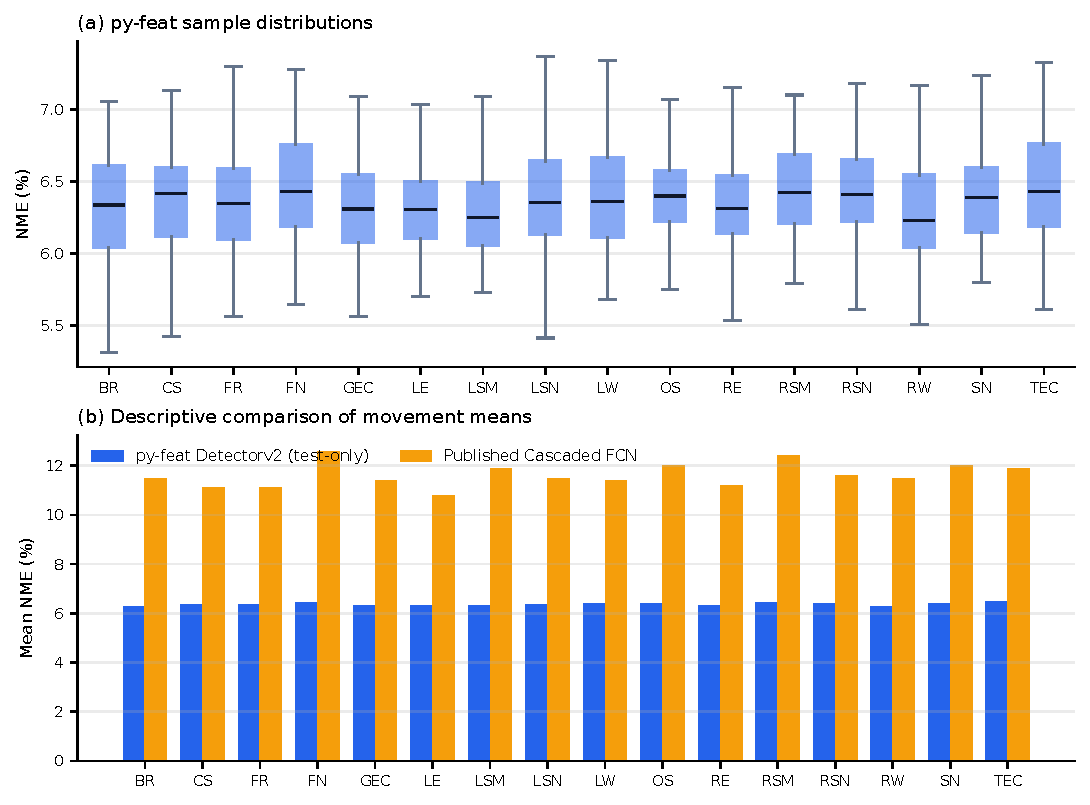
\includegraphics[width=0.97\textwidth]{figures/aflfp_nme.pdf}
\caption{AFLFP landmark localization by movement. (a) Boxplots summarize the
71 test-only samples in each movement; whiskers follow the standard 1.5-IQR
rule and outliers are hidden for legibility. (b) Cohort means are shown beside
the Cascaded FCN means reported by Xia et al. \cite{xia2023aflfp}. The latter
are descriptive references, not matched-split comparisons.}
\label{fig:aflfp}
\end{figure*}

\begin{table*}[t]
\caption{AFLFP NME by movement (\%). Population SD and P90 are computed from
the saved Py-Feat sample predictions. The final column is transcribed from
the published Cascaded FCN row \cite{xia2023aflfp}.}
\label{tab:aflfp-movements}
\centering
\footnotesize
\begin{tabular}{llrrrrrr}
\toprule
Movement & Abbr. & $n$ & Mean & SD & Median & P90 & Cascaded FCN mean \\
\midrule
brow raise & BR & 71 & 6.296 & 0.393 & 6.336 & 6.717 & 11.5 \\
close smile & CS & 71 & 6.350 & 0.395 & 6.415 & 6.802 & 11.1 \\
frown & FR & 71 & 6.372 & 0.408 & 6.346 & 6.944 & 11.1 \\
funny & FN & 71 & 6.448 & 0.398 & 6.431 & 6.937 & 12.6 \\
gentle eyes closure & GEC & 71 & 6.312 & 0.373 & 6.308 & 6.755 & 11.4 \\
left eyebrow & LE & 71 & 6.317 & 0.344 & 6.306 & 6.799 & 10.8 \\
left smile & LSM & 71 & 6.310 & 0.350 & 6.247 & 6.773 & 11.9 \\
left snarl & LSN & 71 & 6.378 & 0.447 & 6.352 & 6.963 & 11.5 \\
left wink & LW & 71 & 6.392 & 0.391 & 6.362 & 6.886 & 11.4 \\
open smile & OS & 71 & 6.396 & 0.305 & 6.398 & 6.764 & 12.0 \\
right eyebrow & RE & 71 & 6.315 & 0.355 & 6.314 & 6.726 & 11.2 \\
right smile & RSM & 71 & 6.429 & 0.404 & 6.424 & 6.916 & 12.4 \\
right snarl & RSN & 71 & 6.416 & 0.402 & 6.410 & 6.842 & 11.6 \\
right wink & RW & 71 & 6.271 & 0.418 & 6.228 & 6.849 & 11.5 \\
snarl & SN & 71 & 6.398 & 0.472 & 6.388 & 6.998 & 12.0 \\
tight eyes closure & TEC & 71 & 6.486 & 0.423 & 6.429 & 7.011 & 11.9 \\
\bottomrule
\end{tabular}

\end{table*}

\Cref{fig:aflfp-target} connects the landmark benchmark to the intended
oral-motor measurements. The selected open-smile case has 5.66\% normalized
aperture, compared with 0.29\% in the close-smile case. NME for the four
displayed cases ranges from 6.26\% to 7.44\%. The left/right cases also show
that a single-frame lip-corner height difference is visible but is
pose-sensitive and should be confirmed over a sequence.

\begin{figure*}[t]
\centering
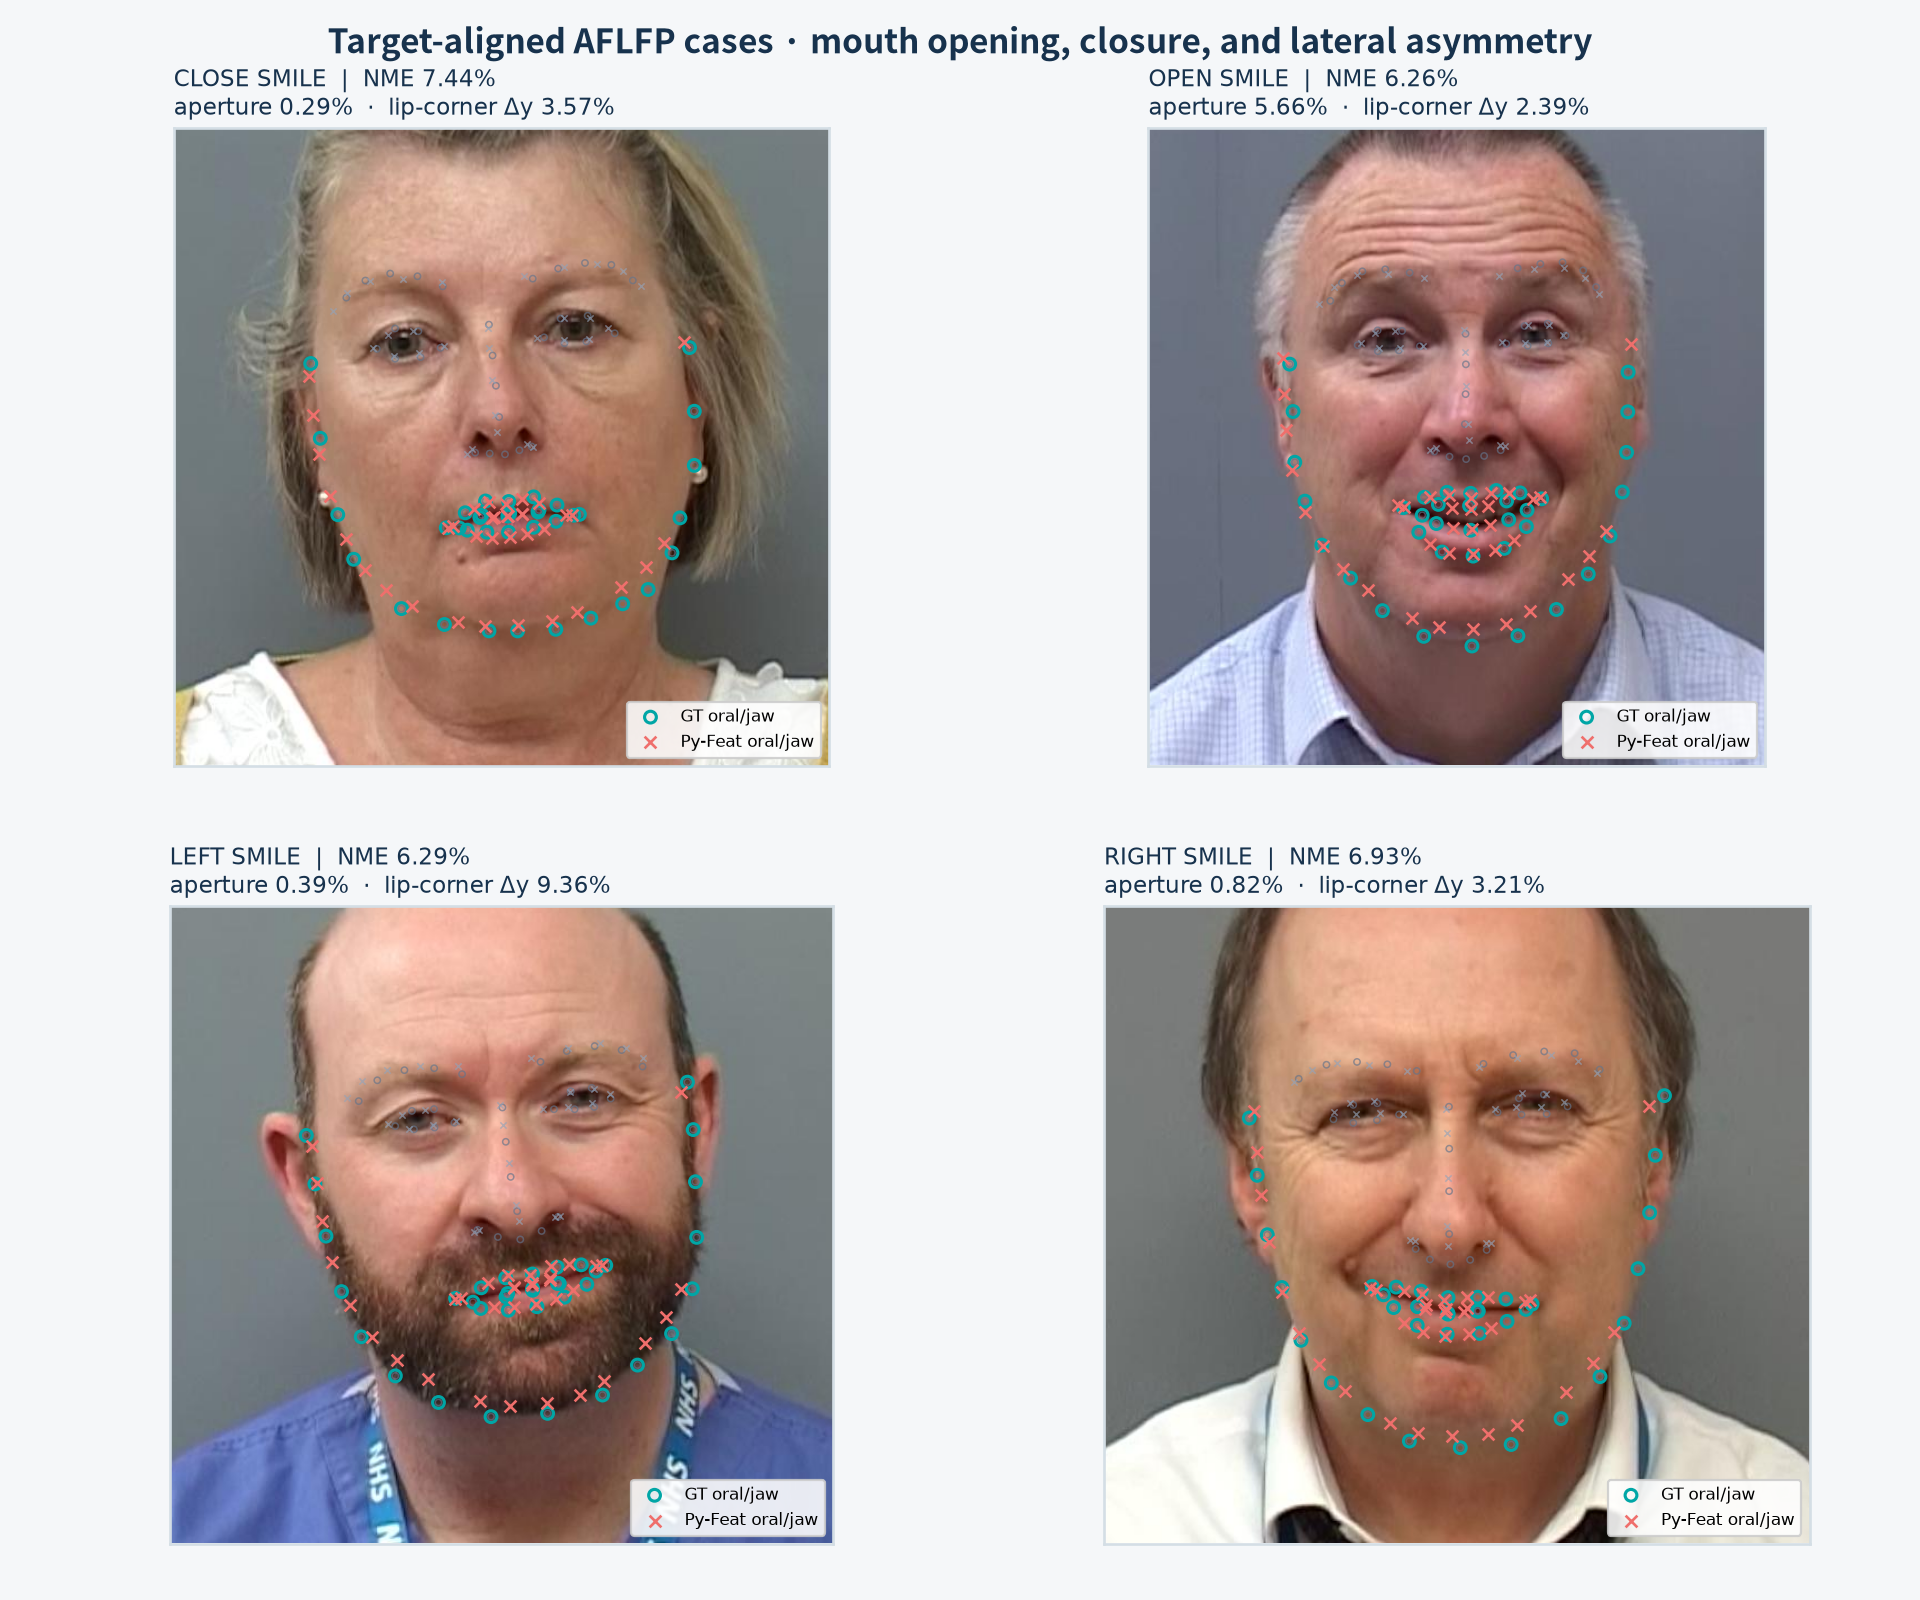
\includegraphics[width=0.84\textwidth]{figures/aflfp_target_landmarks.png}
\caption{Target-aligned AFLFP landmark cases. Gray marks show all 68 points;
teal circles and coral crosses emphasize ground-truth and Py-Feat oral/jaw
points. The panels cover mouth closure, mouth opening, and left/right
lip-corner movement. NME and exploratory normalized oral geometries are shown
for each publication-eligible case.}
\label{fig:aflfp-target}
\end{figure*}

\subsection{DISFA Action Units}

All \DISFASamples{} selected frames yield finite AU predictions
(\DISFADetection{} detection). Macro F1 is \DISFAFOne{} and macro ICC(3,1)
is \DISFAICC{}, with warm throughput of \DISFAFPS{} FPS. AU performance is
heterogeneous (\cref{fig:disfa-metrics,tab:disfa-aus}). The strongest F1
values occur for AU25 (0.959), AU02 (0.917), and AU04 (0.878). The weakest
occur for AU20 (0.479), AU17 (0.507), and AU05 (0.548).

Prediction counts expose distinct error modes. AU05 has 59 positives but only
25 predicted positives, and AU20 has 132 versus 85, consistent with
under-detection. Conversely, AU17 has 282 positives but 780 predicted
positives, and AU12 has 671 versus 1,123, consistent with over-detection at
the fixed threshold. These count asymmetries explain why a single macro score
is insufficient.

\begin{figure*}[t]
\centering
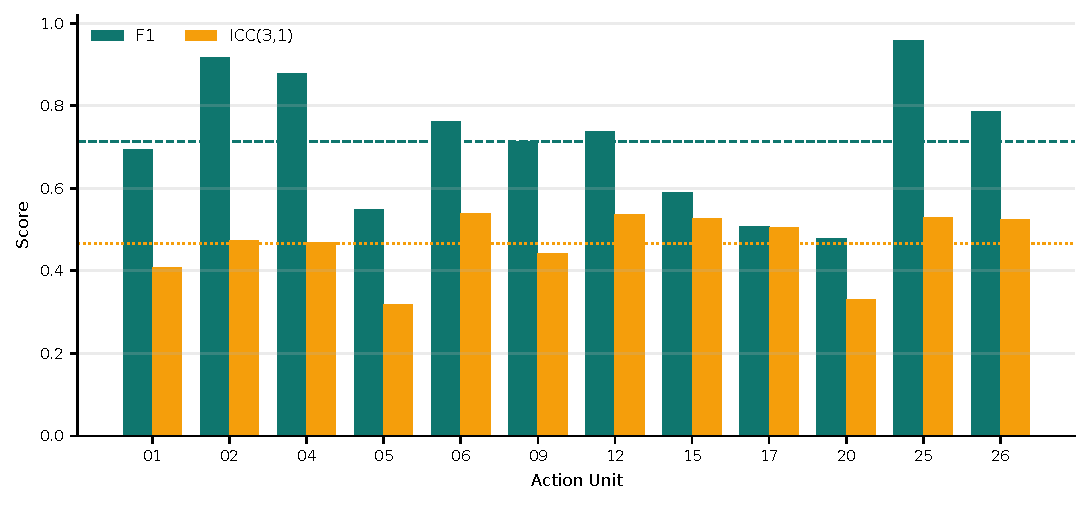
\includegraphics[width=0.93\textwidth]{figures/disfa_au_metrics.pdf}
\caption{DISFA per-AU F1 and ICC(3,1). Dashed and dotted horizontal lines are
the respective macro means. F1 is the primary presence metric; ICC is
auxiliary because the 0--5 ground-truth intensity and 0--1 Py-Feat output are
not calibrated to a common scale.}
\label{fig:disfa-metrics}
\end{figure*}

Across the 12 AUs, positive prevalence and F1 have a descriptive Pearson
correlation of
$r=\DISFAPrevalenceCorrelation$. The pattern is compatible with more stable
measurement when more positives are available, but it does not establish a
causal effect: AU identity, visual distinctiveness, co-activation, and model
training frequency are confounded. AU05, for example, has only 59 positive
frames (1.09\%), whereas AU25 has 1,497 (27.72\%).

\begin{table*}[t]
\caption{DISFA test-only results by AU. Positive support uses intensity
$\geq 2$; predicted positives use score $\geq 0.5$. Each AU is evaluated on
5,400 finite prediction/label pairs.}
\label{tab:disfa-aus}
\centering
\small
\begin{tabular}{lrrrrr}
\toprule
AU & Positive support & Prevalence (\%) & Predicted positive & F1 & ICC(3,1) \\
\midrule
AU01 & 299 & 5.54 & 389 & 0.695 & 0.409 \\
AU02 & 261 & 4.83 & 245 & 0.917 & 0.472 \\
AU04 & 800 & 14.81 & 934 & 0.878 & 0.469 \\
AU05 & 59 & 1.09 & 25 & 0.548 & 0.318 \\
AU06 & 409 & 7.57 & 590 & 0.763 & 0.539 \\
AU09 & 208 & 3.85 & 237 & 0.715 & 0.442 \\
AU12 & 671 & 12.43 & 1,123 & 0.737 & 0.536 \\
AU15 & 100 & 1.85 & 198 & 0.591 & 0.527 \\
AU17 & 282 & 5.22 & 780 & 0.507 & 0.504 \\
AU20 & 132 & 2.44 & 85 & 0.479 & 0.331 \\
AU25 & 1,497 & 27.72 & 1,606 & 0.959 & 0.528 \\
AU26 & 440 & 8.15 & 571 & 0.785 & 0.525 \\
\bottomrule
\end{tabular}

\end{table*}

\Cref{fig:disfa-target} shows the target outputs on actual DISFA frames.
The AU12 case has manual intensity 5 and Py-Feat probability 1.00; the AU25
case has 5 and 1.00; and the strongest sampled AU26 case has 3 and 0.99.
The target-inactive reference produces 0.00 for all three probabilities.
Co-activation is visible in the positive cases, reinforcing that AU12,
AU25, and AU26 should be analyzed jointly rather than as mutually exclusive
labels.

\begin{figure*}[t]
\centering
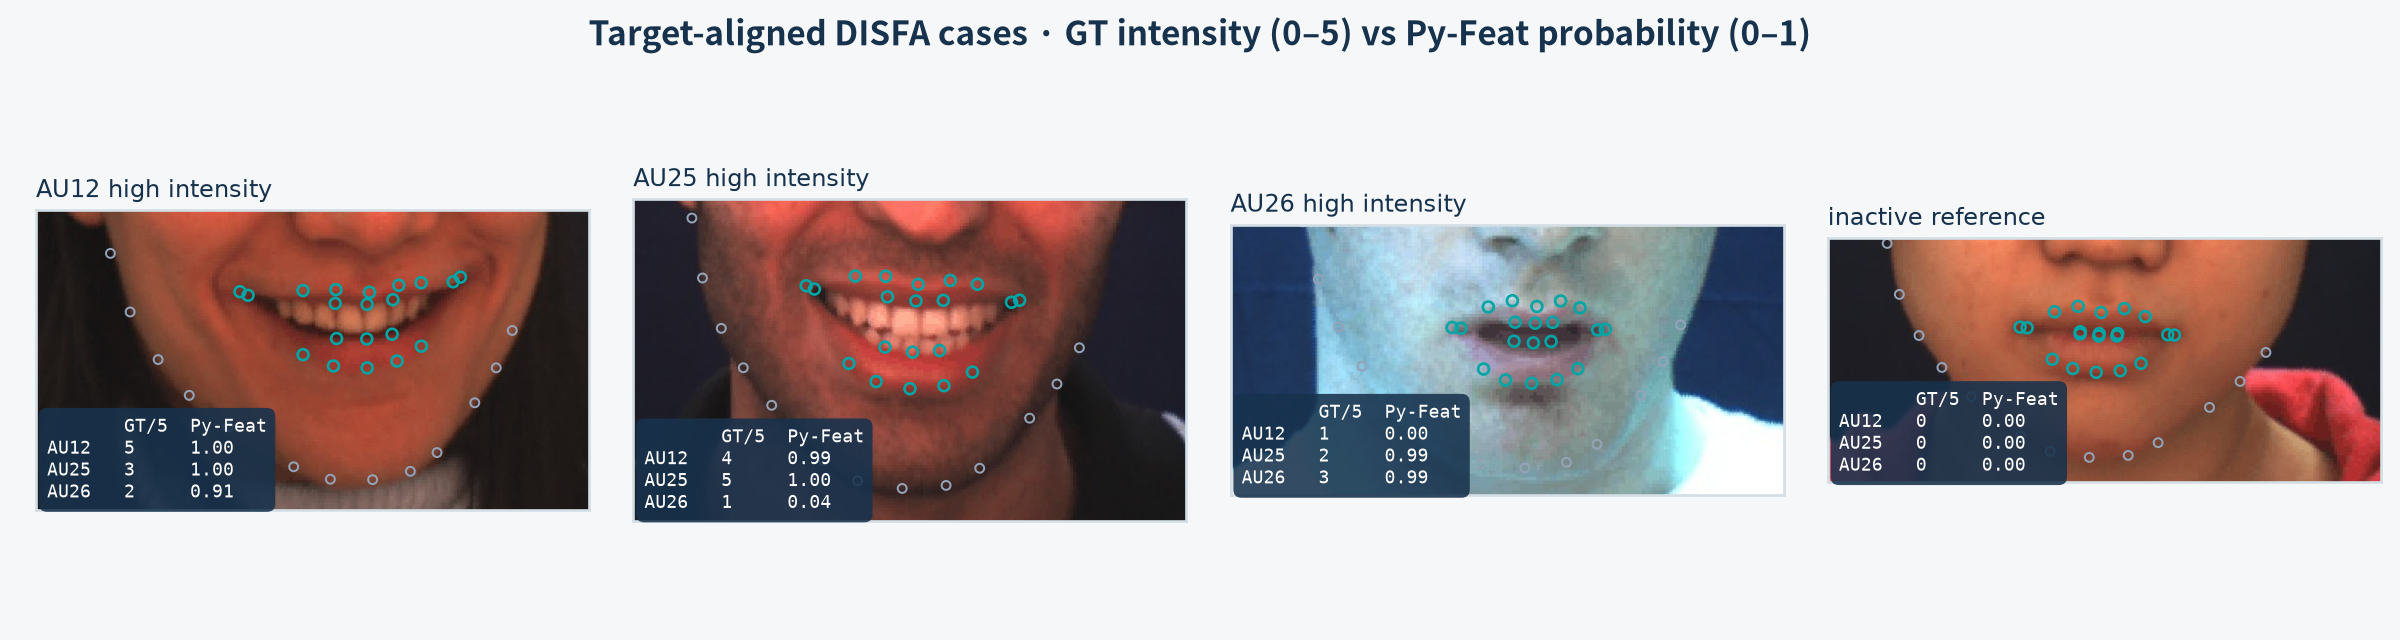
\includegraphics[width=0.97\textwidth]{figures/disfa_target_aus_strip.png}
\caption{Target-aligned DISFA cases for AU12 (lip-corner pull), AU25 (lips
part), AU26 (jaw drop), and a target-inactive reference. Teal points are the
Py-Feat mouth landmarks and gray points trace the jaw. The inset compares
manual intensity (GT, 0--5) with Py-Feat probability (0--1); the scales are
not calibrated. These deliberately clear high-intensity examples are
qualitative and are not estimates of cohort-level performance.}
\label{fig:disfa-target}
\end{figure*}

\section{Discussion}

The landmark result is the clearest evidence of cross-domain utility.
Detectorv2 detects every selected AFLFP face and keeps movement means within a
narrow interval, despite facial asymmetry and movement-specific deformation.
Its 6.368\% mean NME is also substantially below the 11.6\% historical
Cascaded FCN reference. The comparison should motivate a matched, full-corpus
replication, not a leaderboard claim: the older baseline was trained and
evaluated under a different protocol.

The DISFA result is more nuanced. Macro F1 0.714 indicates useful zero-shot AU
presence detection, but the 0.480 range between the best and worst AUs is
large. Prevalence and predicted-positive counts show both data scarcity and
threshold miscalibration. A deployment that treats every AU score identically
would therefore conceal predictable failure modes. Per-AU calibration on a
separate validation population could improve a downstream application, but
doing so would no longer be the test-only setting evaluated here.

The macro ICC of 0.467 should not be read as a direct comparison with
DISFA-trained intensity regressors. Py-Feat scores are bounded to 0--1 while
DISFA intensity spans 0--5, and no scale mapping was learned. The statistic
still reveals ordinal consistency differences across AUs, but an intensity
study should reserve subjects for calibration, map scores to the DISFA scale,
and report the mapping separately.

The case visualizations make the project linkage concrete. AFLFP supplies
observable mouth-opening and lateral-movement geometry, while DISFA supplies
AU12/25/26 activation patterns on actual faces. The current pipeline therefore
provides candidate inputs for oral-opening, closure, and lower-face movement
analysis. It does not yet measure lip speed, periodicity, audio--visual
synchrony, or task-level clinical discrimination; those require continuous
Task 2/5 recordings and participant-level validation.

Warm throughput near 25--26 FPS demonstrates that batched offline processing
is practical on the measured Apple M1 Pro. It does not imply real-time
end-to-end video throughput: camera capture, decoding, transfer, UI rendering,
model initialization, and result serialization are explicitly excluded.

\section{Limitations}

First, both cohorts are deterministic samples rather than full-corpus
evaluations. AFLFP covers 1,136 of 5,328 paired annotations and DISFA covers
5,400 of 130,814 labeled frames. Subject and target coverage reduce sampling
bias but cannot remove it; one seed also does not quantify sampling
variability. Second, the AFLFP released file inventory differs from the image
count described in the source paper, so the present result is tied to the
inspected local distribution.

Third, test-only execution prevents local leakage through fitting or tuning
but cannot prove that upstream model-development data were disjoint from
these benchmarks. Fourth, the DISFA protocol evaluates independent frames
from the left camera and ignores temporal structure. JPEG materialization may
also cause small score changes near the 0.5 threshold. Fifth, AU F1
binarizes an ordinal task and ICC compares unmatched score ranges. Finally,
AFLFP performance is not clinical validation; landmark accuracy alone does
not establish safety or diagnostic utility for facial palsy. The four
target-aligned cases per dataset are selected to expose the intended signals,
not to represent their population distributions, and their static geometry
is sensitive to head pose.

\section{Reproducibility and Data Governance}

The repository retains benchmark commands, aggregate JSON, sample-level CSV,
generated table fragments, vector figures, software versions, and this
LaTeX source. Running \code{make pdf} validates the saved outputs, regenerates
the aggregate derived assets, and compiles the manuscript. Raw AFLFP and
DISFA media remain excluded because access and redistribution are governed by
their respective dataset terms. The manuscript includes only the selected
publication figures: AFLFP cases are restricted to subjects permitted for
academic publication, and DISFA is shown as target-focused face-region crops.
The target-case manifest stores selection keys, outputs, and coordinates but
no raw media. No clinical or hospital participant data were used, and no new
human-participant data were collected.

\section{Conclusion}

Under a frozen, test-only protocol, Py-Feat Detectorv2 provides complete face
detection and consistent landmark localization on the sampled AFLFP cohort,
with mean NME \AFLFPNMEMean{}. On subject-balanced DISFA frames it reaches
macro F1 \DISFAFOne{}, but AU-specific results vary widely and raw
intensity consistency remains limited. The practical conclusion is
task-dependent: Py-Feat is a strong external landmark baseline here, while AU
deployment requires per-class inspection and, when permitted, independent
calibration. The released result chain makes both findings directly
auditable.

\balance
\begingroup
\sloppy
\bibliographystyle{IEEEtran}
\bibliography{references}
\endgroup

\end{document}
